
运用微元控制体推导流体动力学微分型方程的一个例子:

使用柱坐标系下的微元控制体推导连续性方程,如图\ref{fig:61D}
\begin{figure}[!ht]
 \centering
 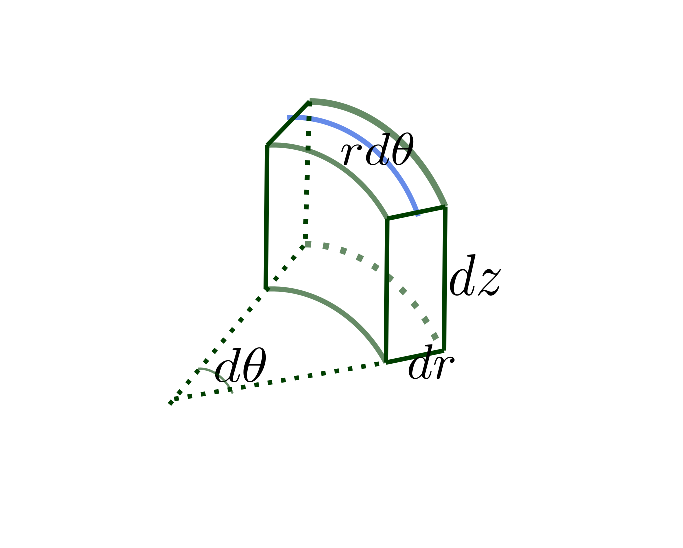
\includegraphics[width=5cm]{differentialControlElement.eps}
 \caption{柱坐标微元控制体}\label{fig:61D}
\end{figure}

对于该微元质量体,$\Delta t$时间内质量变化为
\begin{equation}\label{eq:61cm}
\Delta m = \frac{\partial}{\partial t}(\rho (rd\theta) dr dz)\Delta t
\end{equation}
分别考虑微元质量体六个面的流量,$drdz$确定的两个面分别是左面(可见)与右面。

左面$\Delta t$时间流入量:

\begin{align}\notag
Q_l= & \rho(v_{\theta-\frac{d\theta}{2}}drdz)\Delta t \\
=& (\rho v_{\theta}drdz-\frac{\partial}{\partial \theta}(\rho v_{\theta} drdz)\frac{d\theta}{2})\Delta t
\end{align}
同理得微元体右面$\Delta t$时间流出量
\begin{equation}
Q_r=  (\rho v_{\theta}drdz+\frac{\partial}{\partial \theta}(\rho v_{\theta} drdz)\frac{d\theta}{2})\Delta t \\
\end{equation}
因此微元体左右两个面的净流出量为:
\begin{equation}\label{eq:61crl}
Q_r-Q_l= \frac{\partial}{\partial \theta}(\rho v_{\theta} drdz)d\theta\Delta t
\end{equation}
微元体$rd\theta,dz$确定的前面(可见)和后面的净流出量为:
\begin{align}\notag
Q_b-Q_f =& \rho(v_{r+\frac{dr}{2}}(r+\frac{dr}{2})d\theta dz)\Delta t-\rho(v_{r-\frac{dr}{2}}(r-\frac{dr}{2})d\theta dz)\Delta t\\
=& \frac{\partial }{\partial r}(\rho v_r r d\theta dz)\Delta t\label{eq:61cbf}
\end{align}
同理微元体$rd\theta,dr$确定的上面(可见)和下面的净流出量为:
\begin{equation}\label{eq:61cud}
Q_u-Q_d= \frac{\partial }{\partial z}(\rho v_r rd\theta dr)\Delta t
\end{equation}
根据微元控制体质量守恒,可以得到:
\begin{equation}
-\Delta m=(Q_r-Q_l)+(Q_b-Q_f)+(Q_u-Q_d)
\end{equation}
代入(\ref{eq:61cm},\ref{eq:61crl},\ref{eq:61cbf},\ref{eq:61cud})四个式子得
\begin{align}\notag
-\frac{\partial }{\partial t}(\rho r)=&\frac{\partial }{\partial \theta}(\rho v_{\theta})+
\frac{\partial }{\partial r}(\rho v_r r)+\frac{\partial }{\partial z}(\rho v_z r)\\
\iff & \frac{\partial \rho}{\partial t}+\frac{1}{r}\frac{\partial (\rho v_{\theta})}{\partial \theta}+
\frac{\partial (\rho v_r)}{\partial r}+\frac{\rho v_r}{r}+\frac{\partial(\rho v_z) }{\partial z}=0\label{eq:61cce}
\end{align}
\eqref{eq:61cce}式也可直接从\eqref{eq:52Conti}中利用$\nabla$算子的柱坐标的表达式\eqref{eq:52nablacy}式直接求出。

流体的静力学考虑$\v{v}=\v{0}$,由于流体静止,应变率为零,
因此应力张量$T_{ij}=-p\delta_{ij}$,由\eqref{eq:52Momen}式可以得到流体的静力平衡方程为:
\begin{equation}\label{eq:61static}
\nabla p = \rho \v{f}
\end{equation}
上式两边求旋度得到\eqref{eq:61static}式成立的必要条件:
\begin{equation}\label{eq:61staticNecess}
\nabla \times (\rho \v{f})=\v{0}
\end{equation}
\newglossaryentry{barotropic}
{
  name=正压流体,
  description={$\rho=\rho(p)$,即密度只与压力有关}
}
若\glsdesc{barotropic},那么称流体为\gls{barotropic},在这种情况下$\nabla \rho=\frac{d\rho}{dp}\nabla p$,
因此\eqref{eq:61staticNecess}式化简为:
\begin{align}
&\nabla \rho \times \v{f} + \rho \nabla \times \v{f} =  \v{0}\label{eq:61staticExpand}\\
\Rightarrow & \frac{d\rho}{dp}\nabla p \times \frac{\nabla p}{\rho} + \rho \nabla \times \v{f} =  \v{0}\nonumber\\
\Rightarrow  &  \nabla \times \v{f} =  \v{0}\label{eq:61barotropic}
\end{align}
即对于处于静止状态的正压流体,体积力是有势场。
我们可以说明\eqref{eq:61barotropic}式也是正压流体的充分条件,即在静力平衡方程的基础上,如果有\eqref{eq:61barotropic}式
成立,那么$\rho$与$p$存在单值映射关系。
\begin{align}
&\nabla \times \v{f} =  \v{0}\nonumber\\
\Rightarrow & \nabla \times \frac{\nabla p}{\rho} =  \v{0}\nonumber\\
\Rightarrow  &   \nabla \frac{1}{\rho} \times \nabla p =  \v{0}\label{eq:61parallel}
\end{align}
由\eqref{eq:61parallel}可得到关于$\nabla \frac{1}{\rho}$各阶分量的一阶PDE,附加适当的边界条件可以得到$\frac{1}{\rho}$关于
$\nabla p$和边界条件的解。因此$\frac{1}{\rho}$与$p$的地位在\eqref{eq:61parallel}式是对等的,所以我们可以得到$\rho$与$p$存在单值映射关系。

对于一般的情形,若流体静止,对\eqref{eq:61staticExpand}式两边点乘$\v{f}$,\eqref{eq:61staticExpand}式左边第一项得零,因此我们得到
流体静止体积力的一个必要条件为
\begin{equation}
\v{f}\cdot (\nabla \times \v{f})=0
\end{equation}
若外力场是重力场,$\v{f}=-g\v{k}$,对于密度为常量的液体,可以得到
\begin{equation}
p=-\rho g z + p_{z=0}
\end{equation}
如果我们考虑一具有恒定水平加速度$\v{a}=a\v{i}$的非惯性系,并且取坐标原点在自由液面上,则
\begin{equation}
p=-\rho(gz+ax)+p_a
\end{equation}
$p_a$代表大气压,同时由上式可以得到自由液面的形状在惯性系中具有$gz+ax=0$这种倾斜的直线的形状。